\section{Proxy}

O padrão Proxy adiciona uma camada a um 
objeto, permitindo que haja um controle de 
acesso ao mesmo. Qualquer interação com o 
objeto Proxy é repassada para o objeto 
real. Existe mais de uma motivação 
para seu uso, apesar da estrutura do padrão, 
apresentada na figura \ref{proxy_struct},  
permanecer a mesma. Essas motivações 
podem ser divididas em três grupos de 
proxy: remoto, virtual e de proteção. 

Um proxy remoto pode ser utilizado como um 
representante de um objeto, servindo como um 
intermediário e armazenando dados que devem 
ser repassados para o objeto real. Já um 
proxy virtual armazena informações sobre 
um objeto de forma que ele possa ser criado 
apenas quando for necessário, economizando 
espaço ou tempo de execução. Por fim, um 
proxy de proteção pode controlar o acesso 
a um objeto, exigindo que um objeto cliente 
precise cumprir algum requisito antes de 
acessar o objeto real. 

\begin{figure}[htb]
	\caption{\label{proxy_struct}Estrutura do Proxy}
	\begin{center}
	    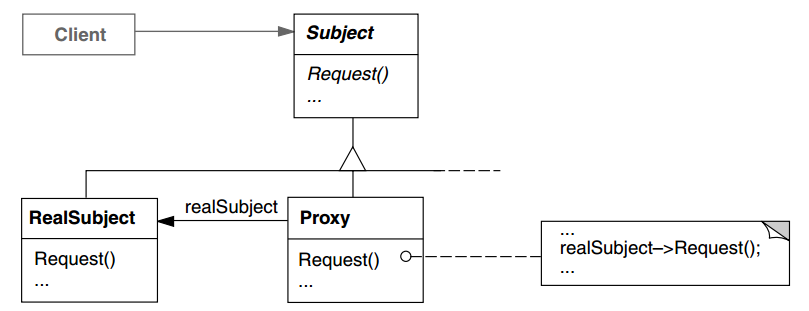
\includegraphics[scale=0.5]{5_padroes-contexto-funcional/5.2_estruturais/5.2.7_proxy/diagram.png}
	\end{center}
\end{figure}

\subsection*{Exemplo Orientado a Objetos}

Como exemplo de Proxy podem ser utilizadas 
imagens que são incluídas em editores de 
texto. É desejado que um documento seja aberto 
rapidamente e o carregamento das imagens 
presentes nele pode causar uma lentidão 
desnecessária. Para isso, é criado um objeto 
Proxy que armazena em seus atributos as 
informações necessárias, como o caminho 
para a imagem e seu posicionamento no 
documento. Quando o documento termina de 
ser aberto, as imagens são carregadas de 
fato através de seus proxys. Esse é um 
exemplo de proxy virtual, seu diagrama de 
classes pode ser visto na imagem \ref{proxy_exemplo} 
e a implementação no código \ref{ooproxy}.

\begin{figure}[htb]
	\caption{\label{proxy_exemplo}Exemplo de Proxy}
	\begin{center}
	    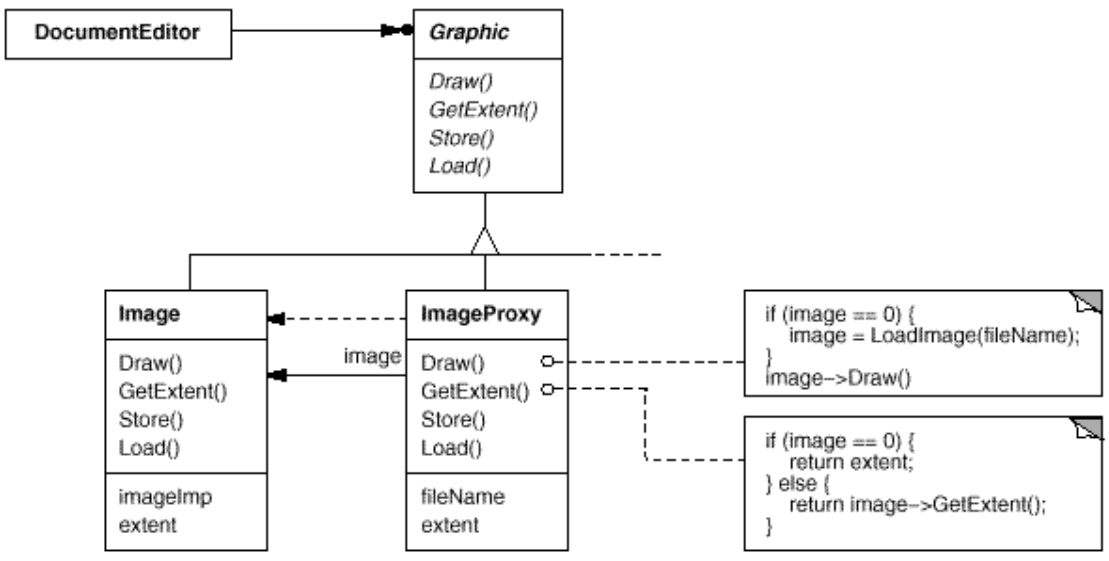
\includegraphics[scale=0.4]{5_padroes-contexto-funcional/5.2_estruturais/5.2.7_proxy/proxy_exemplo.png}
	\end{center}
\end{figure}

\begin{lstlisting}[caption={Proxy Orientado a Objetos},label=ooproxy]

trait Graphic {
	def Draw(point : Point);
	def GetExtent() : Point;
	def Store(ostream : Stream);
	def Load(istream : Stream);
}

class Image() extends Graphic{
	
	var extent : Point;

	def Image(fileName : String) {
		
	}

	def Draw(point : Point){
		// Operação de desenho da imagem
	}

	def GetExtent() : Point {
		return extent;
	}

	def Store(ostream : Stream) {
		// Salva imagem em um arquivo
	}

	def Load(istream : Stream) {
		// Carrega imagem de um arquivo
	}
}

class ImageProxy(var fileName : String, var extent : Point) extends Graphic{

	var image : Image = null;

	def Draw(point : Point){
		if(image == null){
			image = new Image(fileName);
		}
		image.Draw();
	}

	def GetExtent() : Point {
		if(image == null){
			return extent;
		} else {
			return image.GetExtent();
		}
	}

	def Store(ostream : Stream) {
		// Salva imagem em um arquivo
	}

	def Load(istream : Stream) {
		// Carrega imagem de um arquivo
	}

}

\end{lstlisting}

\subsection*{Contexto Funcional}


\begin{lstlisting}[caption={Proxy Funcional},label=fpproxy]
    

    
\end{lstlisting}